
\documentclass[12pt,t]{beamer}
\usepackage{graphicx}
\usepackage{xcolor}
\usepackage{tikz}
\setbeameroption{hide notes}
\setbeamertemplate{note page}[plain]
\usepackage{listings}

% DEFINE COLORS 
	\definecolor{olive}{rgb}{0.3, 0.4, .1}
	\definecolor{fore}{RGB}{249,242,215}
	\definecolor{back}{RGB}{51,51,51}
	\definecolor{title}{RGB}{255,0,90}
	\definecolor{dgreen}{rgb}{0.,0.6,0.}
	\definecolor{gold}{rgb}{1.,0.84,0.}
	\definecolor{JungleGreen}{cmyk}{0.99,0,0.52,0}
	\definecolor{BlueGreen}{cmyk}{0.99,0,0.13,0.2}
	\definecolor{RawSienna}{cmyk}{0,0.72,1,0.45}
	\definecolor{Magenta}{cmyk}{0,1,0,0}


\setbeamercolor{item}{fg=black}
\setbeamercolor{normal text}{fg=black}
\setbeamercolor{background canvas}{bg=white}
\setbeamercolor{title}{fg=black}
\setbeamercolor{subtitle}{fg=Magenta}
\setbeamercolor{author}{fg=BlueGreen}
\setbeamercolor{section in toc}{fg=BlueGreen}
\setbeamercolor{subsection in toc}{fg=red}
\setbeamercolor{frametitle}{fg=Magenta}


%%%%%%%%%%%%%%% TITLE %%%%%%%%%%%%%%%



\title{\Huge Genotype Reconstruction for Diversity Outbred Mice}
\subtitle{\Large A comparison of \texttt{r/qtl2} and \texttt{DOQTL}}
\author{\large John Spaw$^1$\\  Karl Broman$^2$}
%\institute{\normalsize Advised by Karl Broman}
\date{\texttt{github.com/JohnPSpaw}$^1$ \\ \texttt{github.com/kbroman}$^2$}

%%%%%%%%%%%%%%% SLIDES %%%%%%%%%%%%%%%

\begin{document}

\frame{\titlepage}



\section[Outline]{}
%\frame{\tableofcontents}



\section{Genotype Reconstruction and the Diversity Outbred Population}
	% Insert Karl's slides in this section
		%Founders and breeding diagram (explaining DO population)
		%Image of DO genome showing each chromosome
		%Explanation of Hidden Markov Model
		%Diagram explaining reconstruction

	%Mouse full frame image
	\usebackgroundtemplate{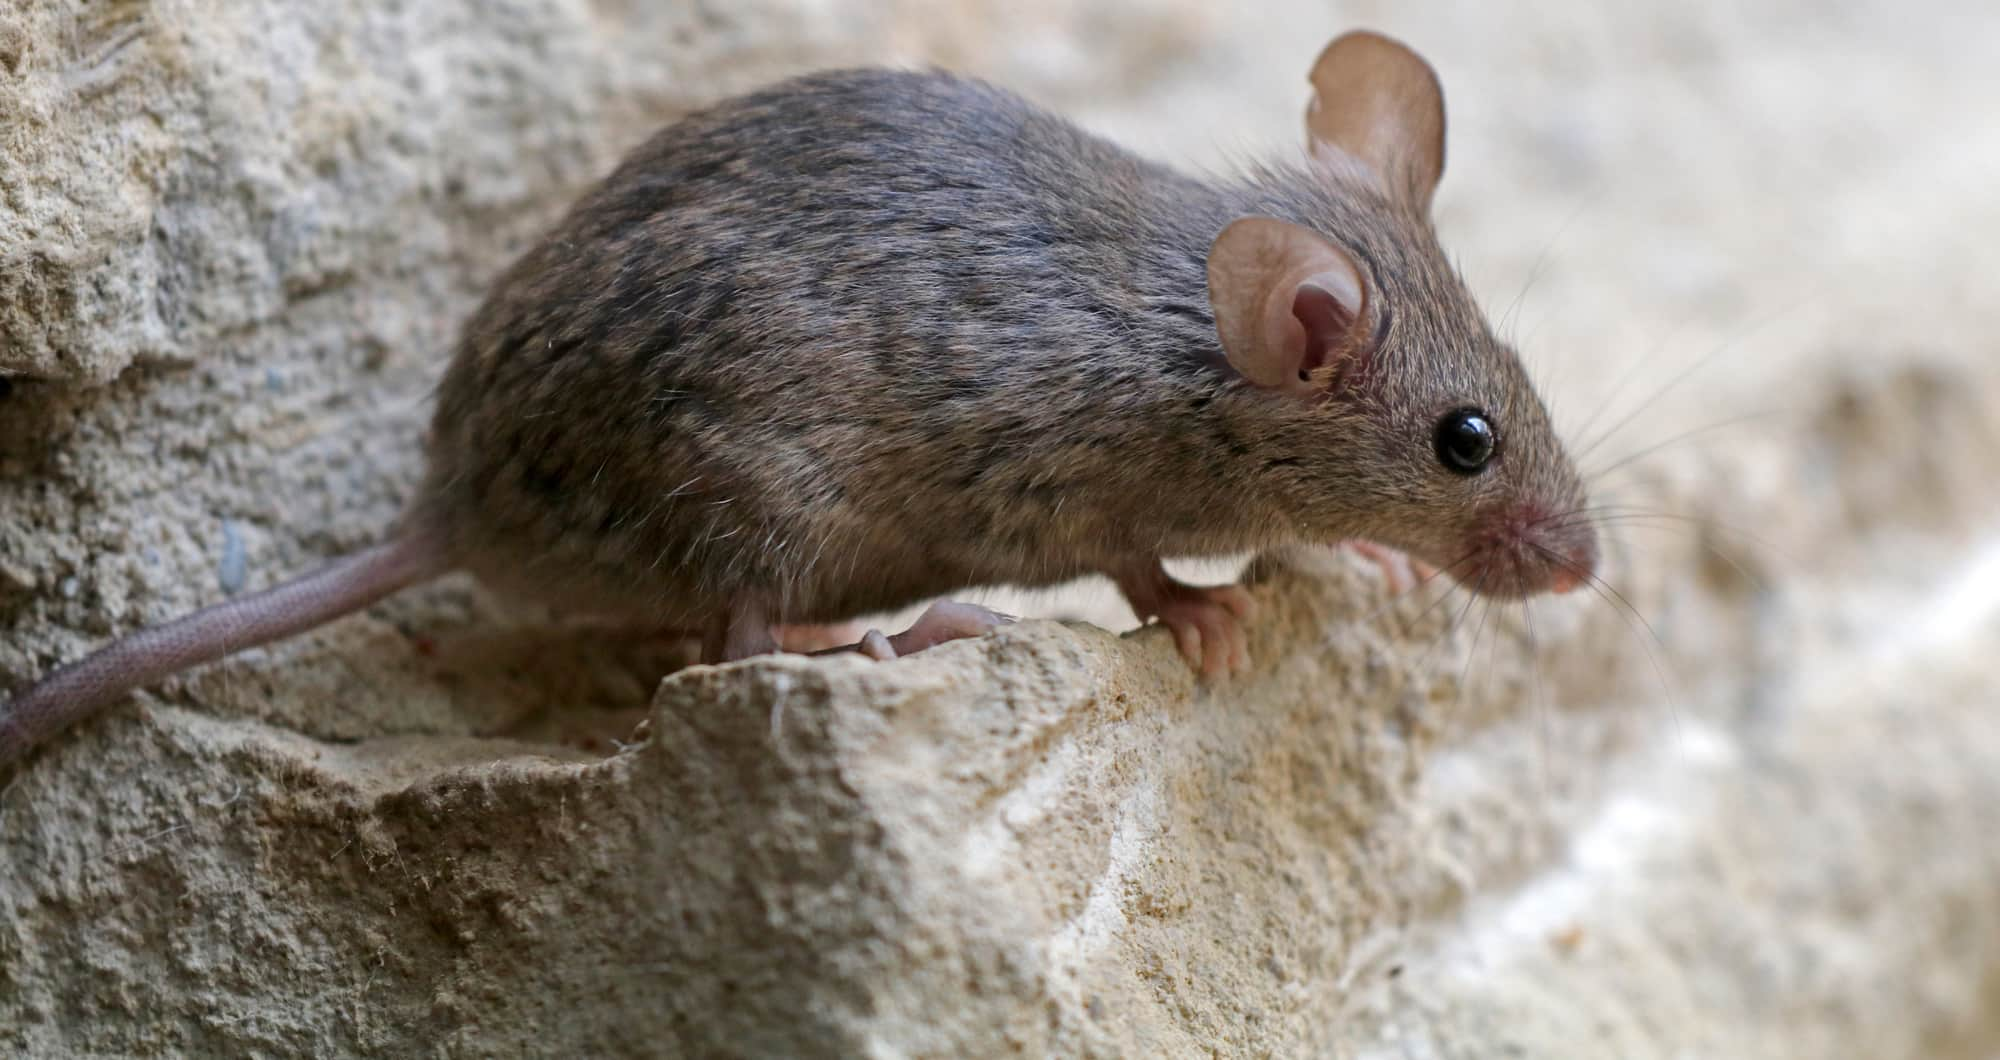
\includegraphics[height=\paperheight,width=\paperwidth]{figures/mouse.jpg}}
	\setbeamertemplate{navigation symbols}{}
    	\begin{frame}[plain]
    	\end{frame}
	
	%DO Cross full frame image
	\usebackgroundtemplate{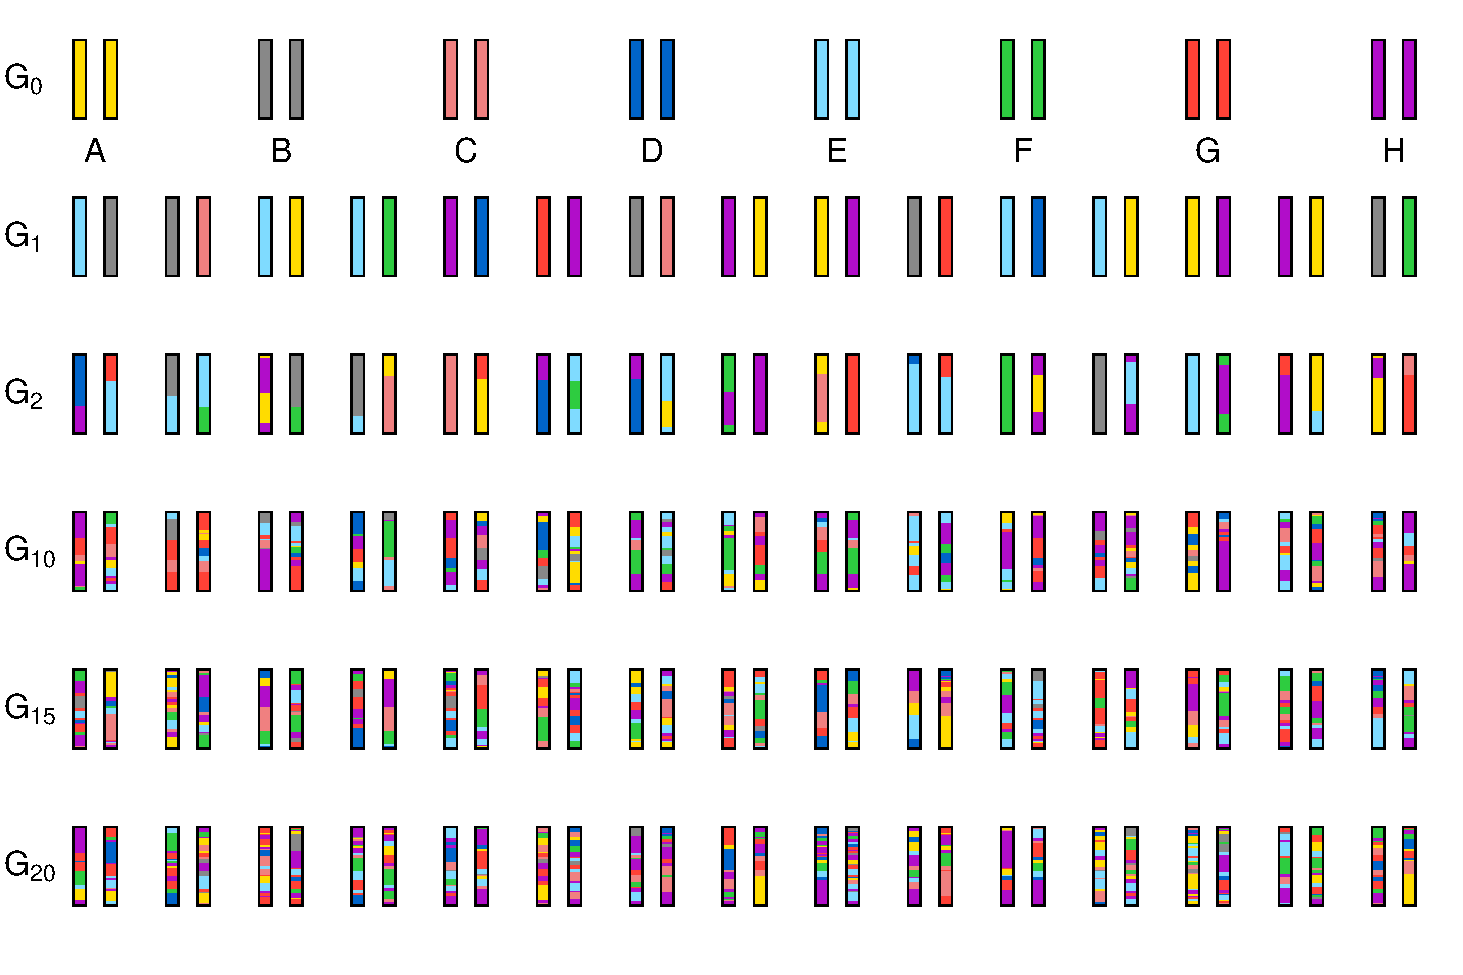
\includegraphics[height=\paperheight,width=\paperwidth]{figures/do_cross.pdf}}
	\setbeamertemplate{navigation symbols}{}
    	\begin{frame}[plain]
    	\end{frame}
		%Re-read DO population overview
		
	%DO Cross full frame image
	\usebackgroundtemplate{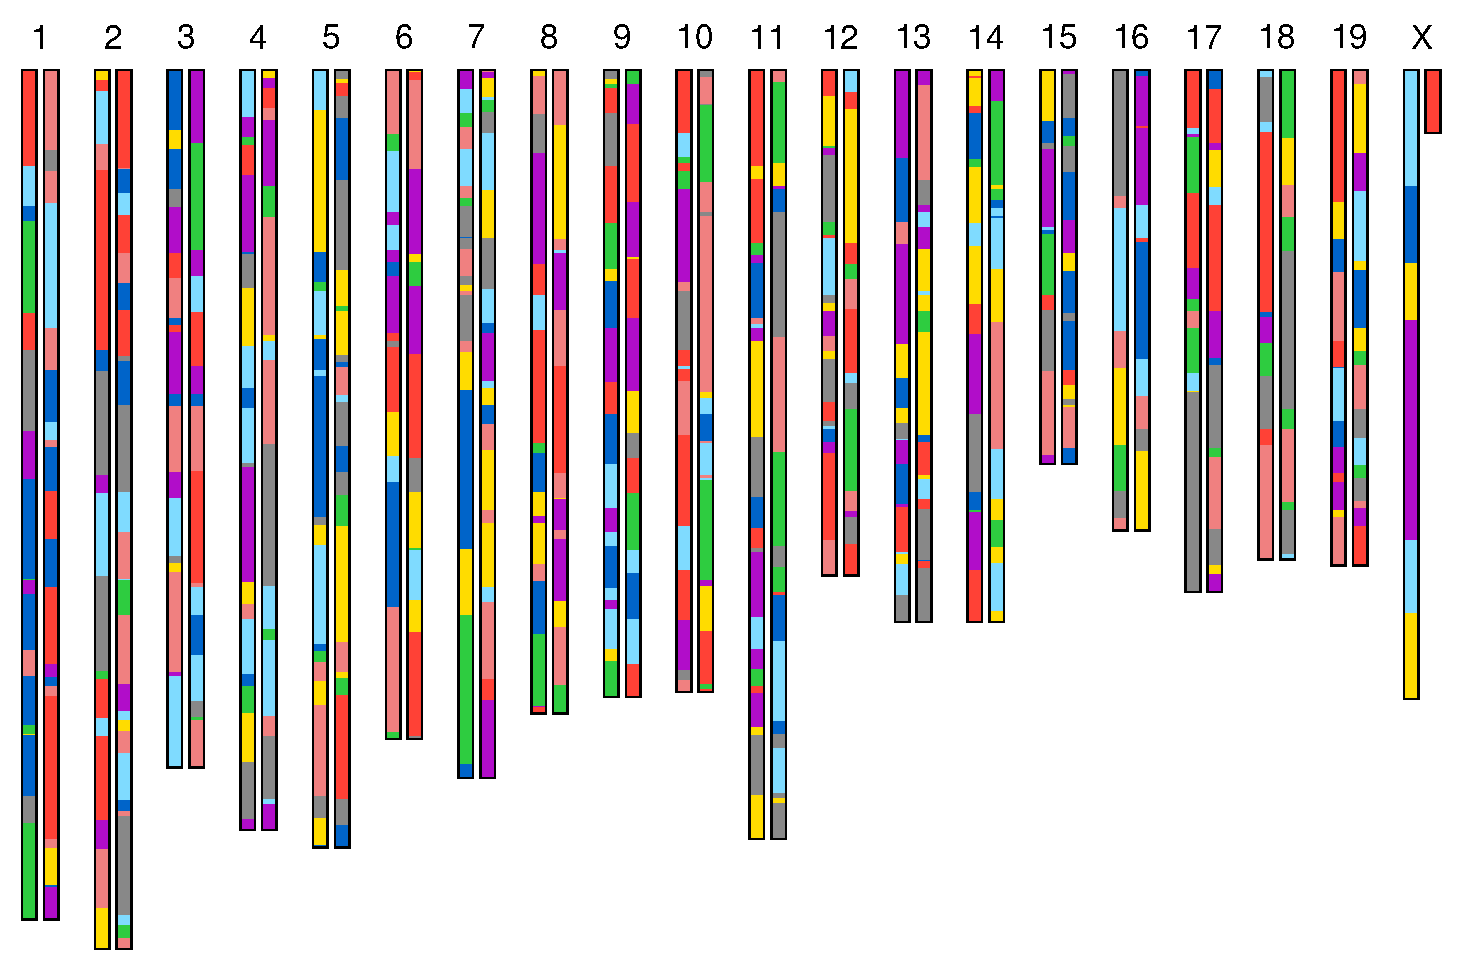
\includegraphics[height=\paperheight,width=\paperwidth]{figures/do_genome.pdf}}
	\setbeamertemplate{navigation symbols}{}
    	\begin{frame}[plain]
    	\end{frame}

	\usebackgroundtemplate{
\includegraphics[height=\paperheight,width=\paperwidth]{figures/white.jpg}}
	\setbeamertemplate{navigation symbols}{}
			
	\begin{frame}
		\frametitle{Hidden Markov Model}
		
		\vspace{0.35in}

		\pause Probabilities are generated from:
		
		\vspace{0.45in}

		
		\begin{enumerate}
				
			\pause \item Transition Model \newline
				%\begin{itemize}
				%	\item Markov Chain with 36 states
				%	\item Probability of transitioning from one diplotype to another
				%\end{itemize} 
			\pause \item \textbf{Emission Model} \\
				%\begin{itemize}
				%	\item Conditional probability distribution of observed data given underlying diplotype state
				%	\item Multinomial distribution over four outcomes (A,B,H,N)
				%\end{itemize} 
		\end{enumerate}
		
		\vspace{0.25in}

		\pause Conditional probability of observed data given underlying diplotype state 
		
	\end{frame}

	%Geno Reconstruction Probs Images
		\usebackgroundtemplate{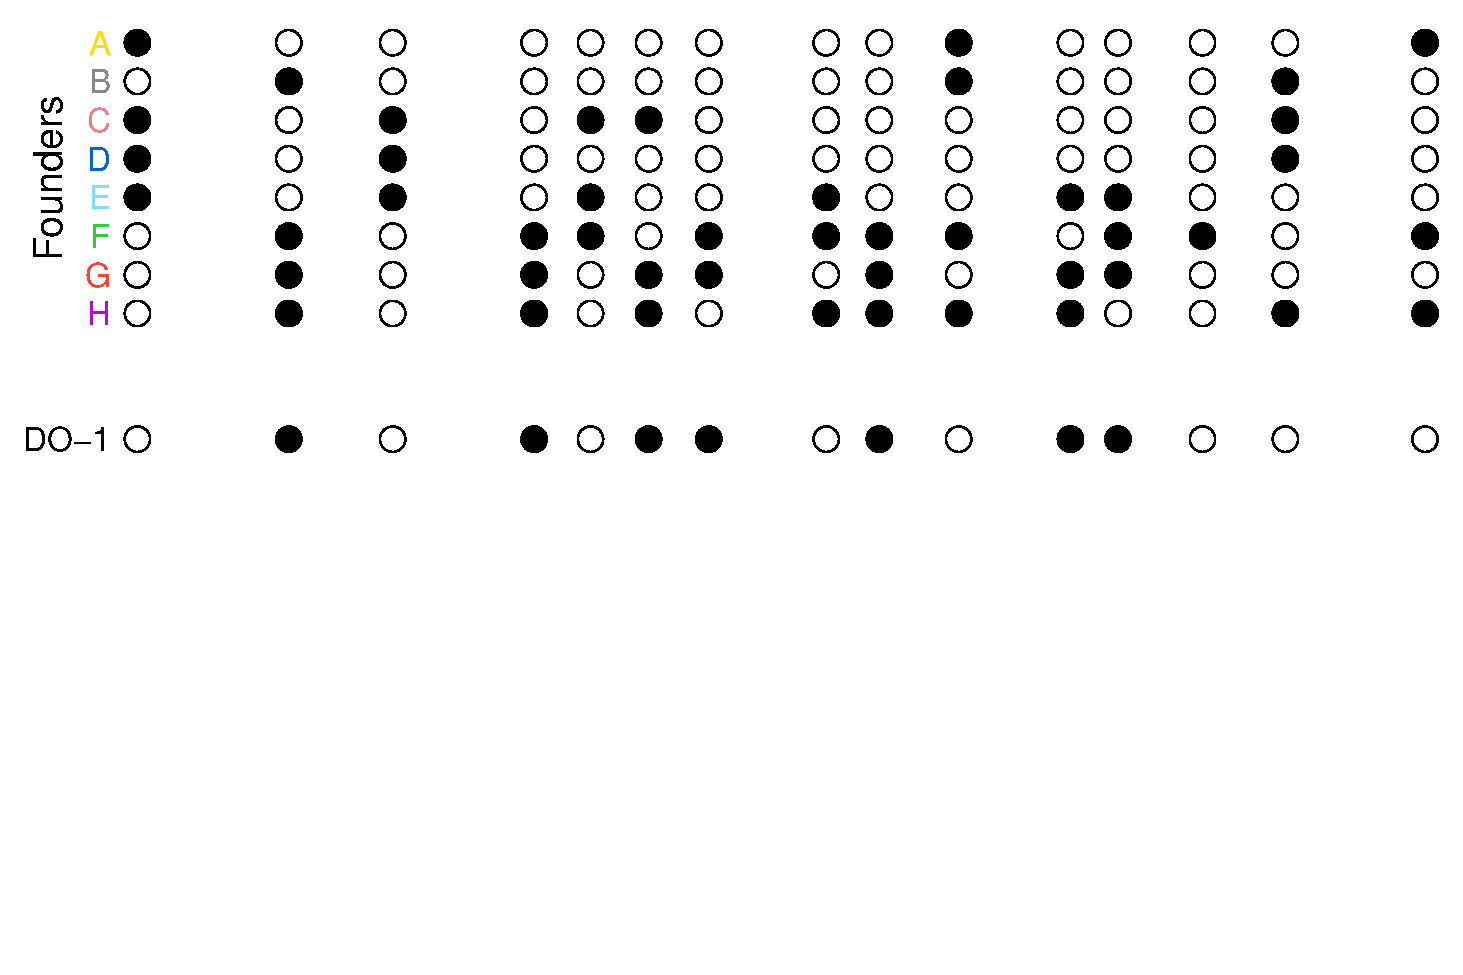
\includegraphics[height=\paperheight,width=\paperwidth]{figures/genoprobsA.pdf}}
		\setbeamertemplate{navigation symbols}{}
    		\begin{frame}[plain]
    		\end{frame}

		\usebackgroundtemplate{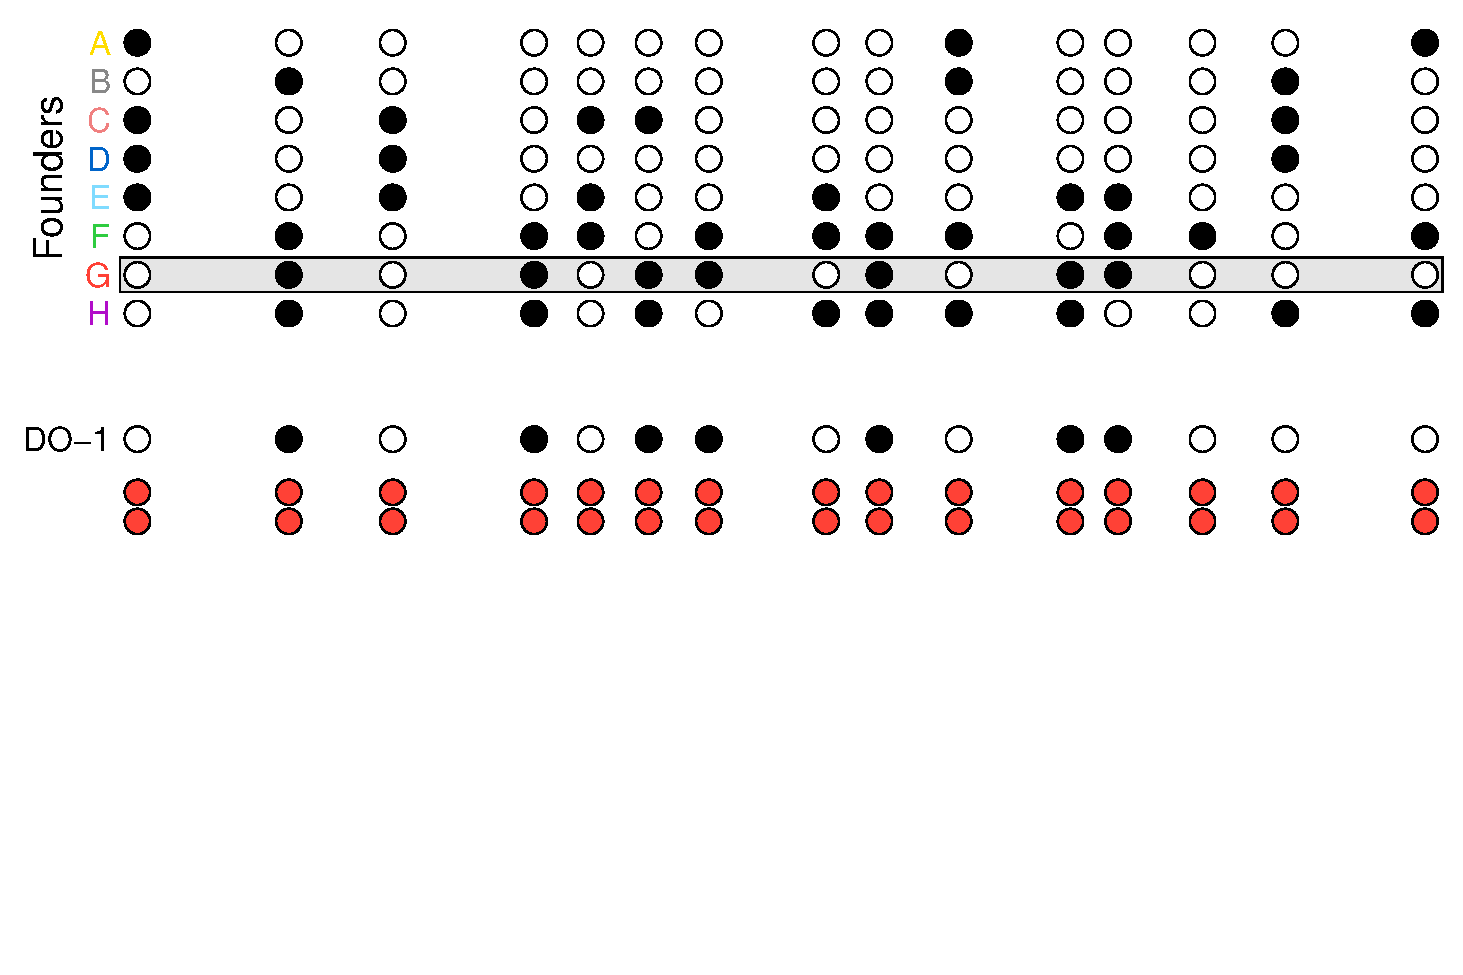
\includegraphics[height=\paperheight,width=\paperwidth]{figures/genoprobsB.pdf}}
		\setbeamertemplate{navigation symbols}{}
    		\begin{frame}[plain]
    		\end{frame}
		
		\usebackgroundtemplate{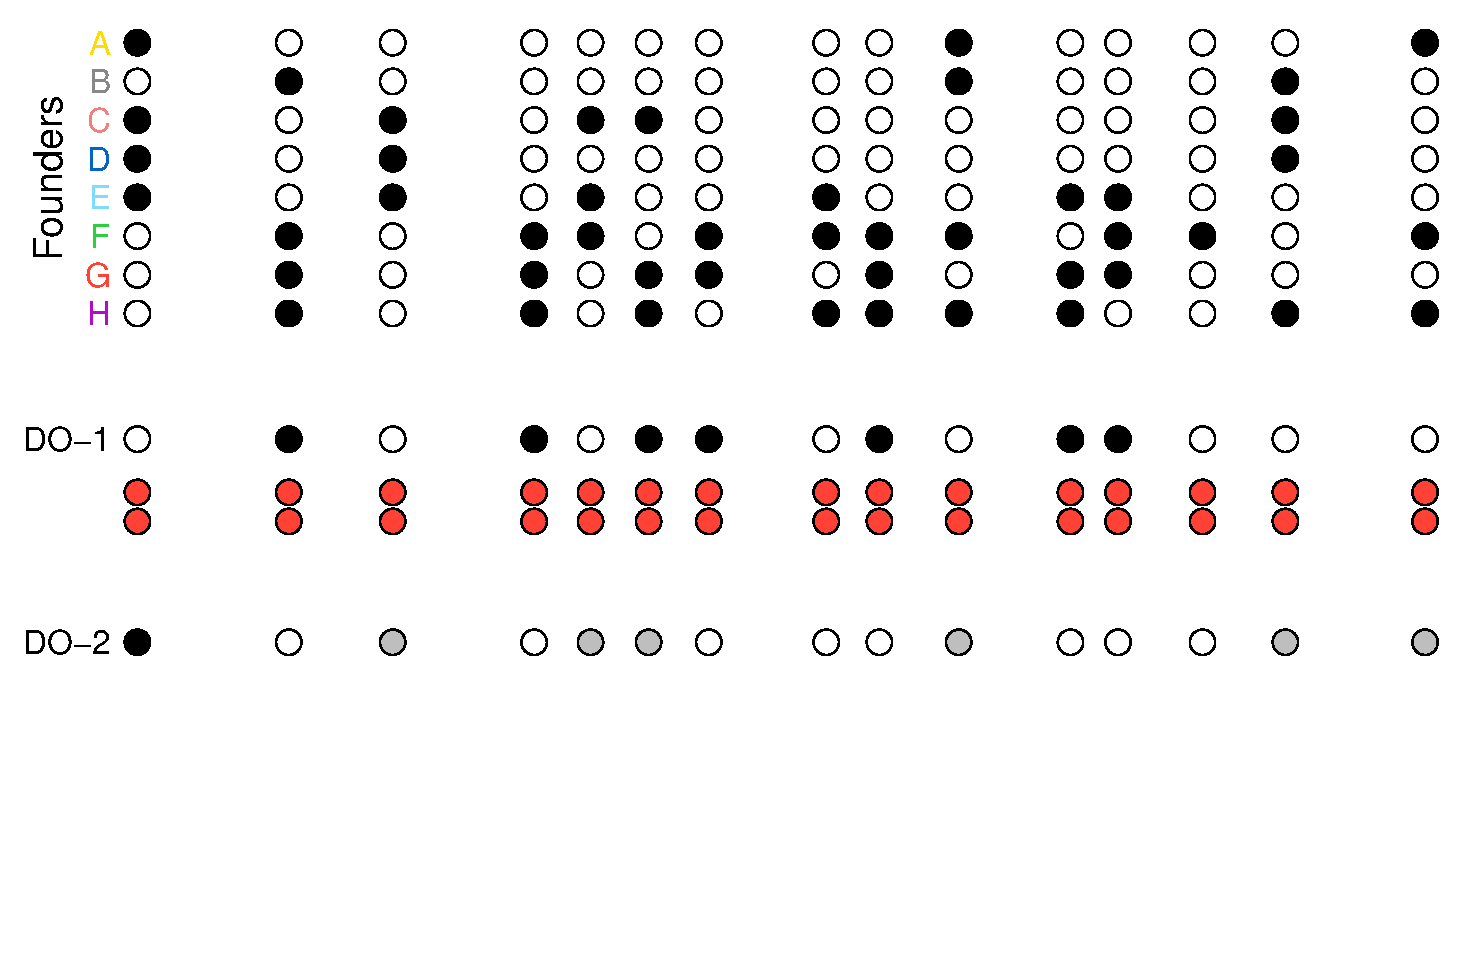
\includegraphics[height=\paperheight,width=\paperwidth]{figures/genoprobsC.pdf}}
		\setbeamertemplate{navigation symbols}{}
    		\begin{frame}[plain]
    		\end{frame}
		
		\usebackgroundtemplate{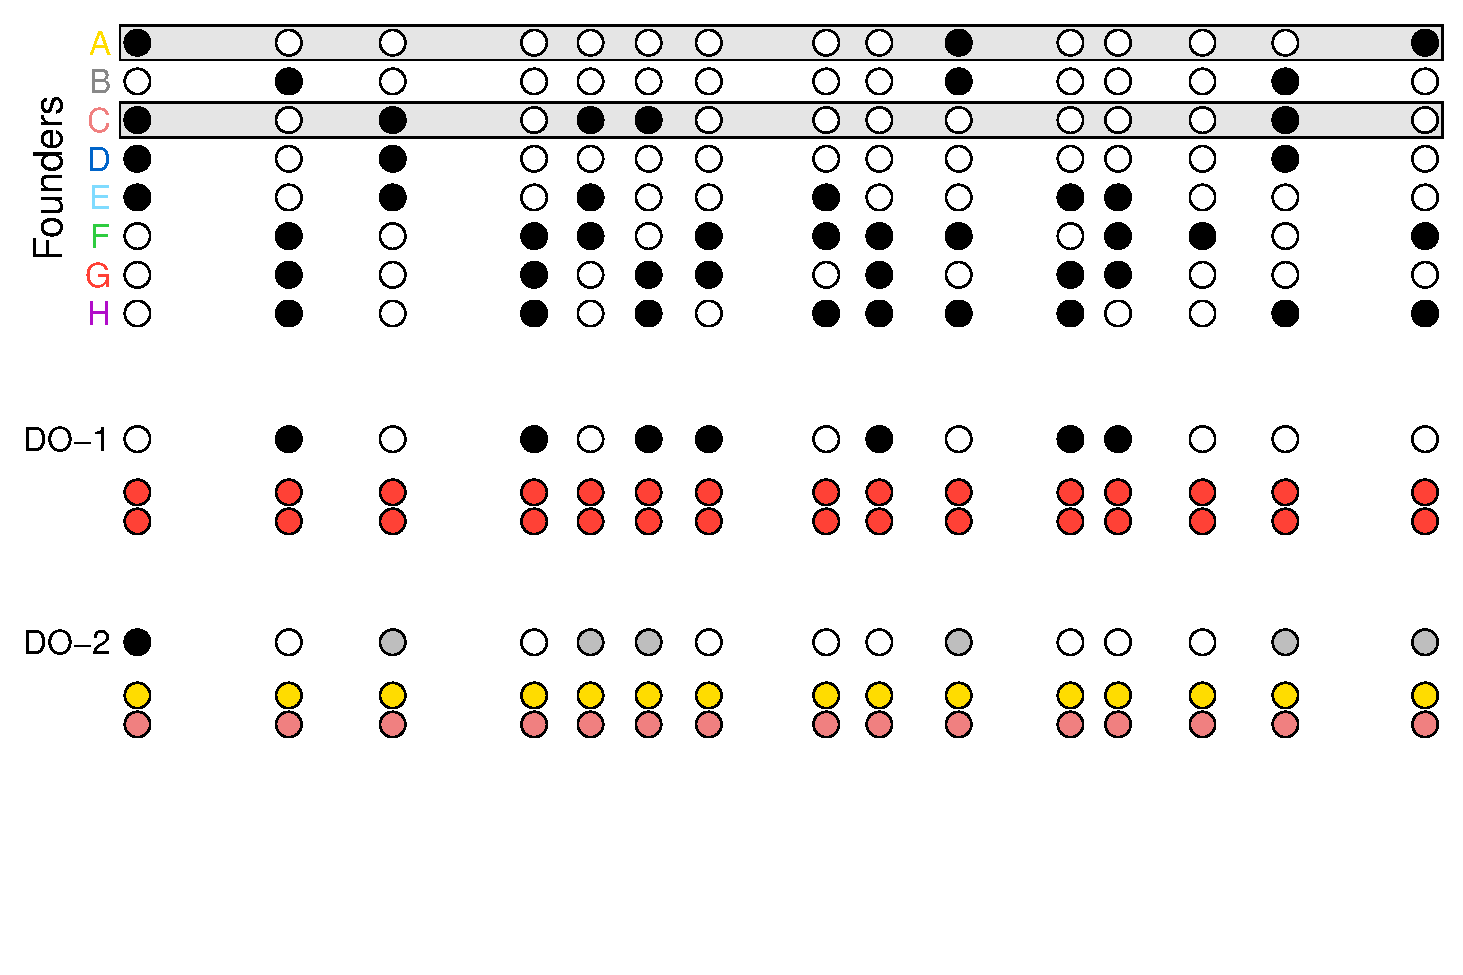
\includegraphics[height=\paperheight,width=\paperwidth]{figures/genoprobsD.pdf}}
		\setbeamertemplate{navigation symbols}{}
    		\begin{frame}[plain]
    		\end{frame}

		\usebackgroundtemplate{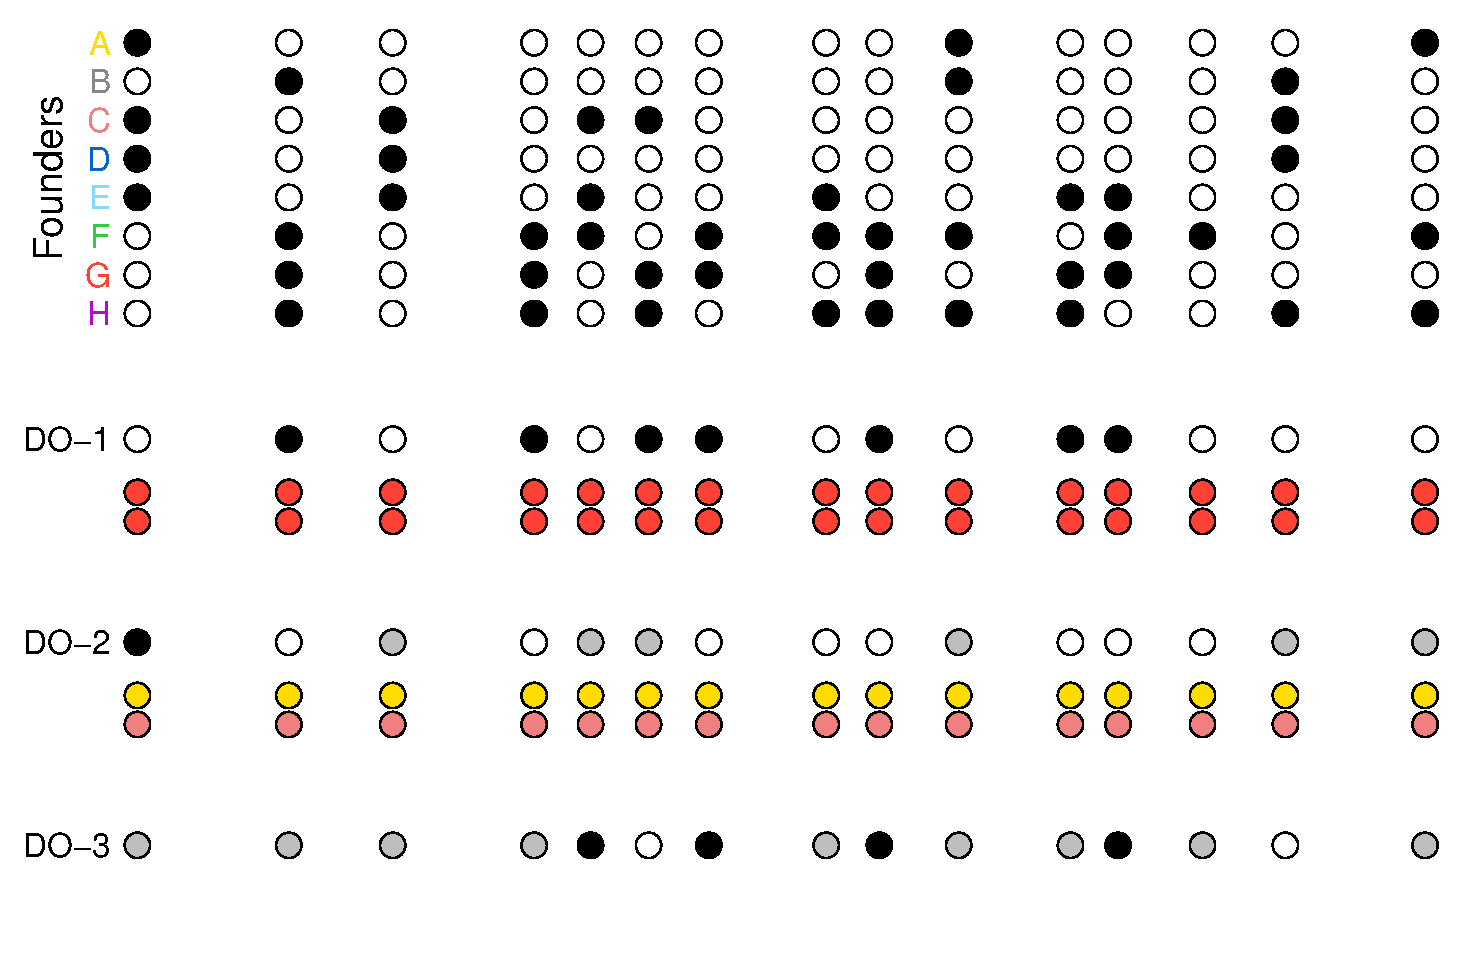
\includegraphics[height=\paperheight,width=\paperwidth]{figures/genoprobsE.pdf}}
		\setbeamertemplate{navigation symbols}{}
    		\begin{frame}[plain]
    		\end{frame}
		
		\usebackgroundtemplate{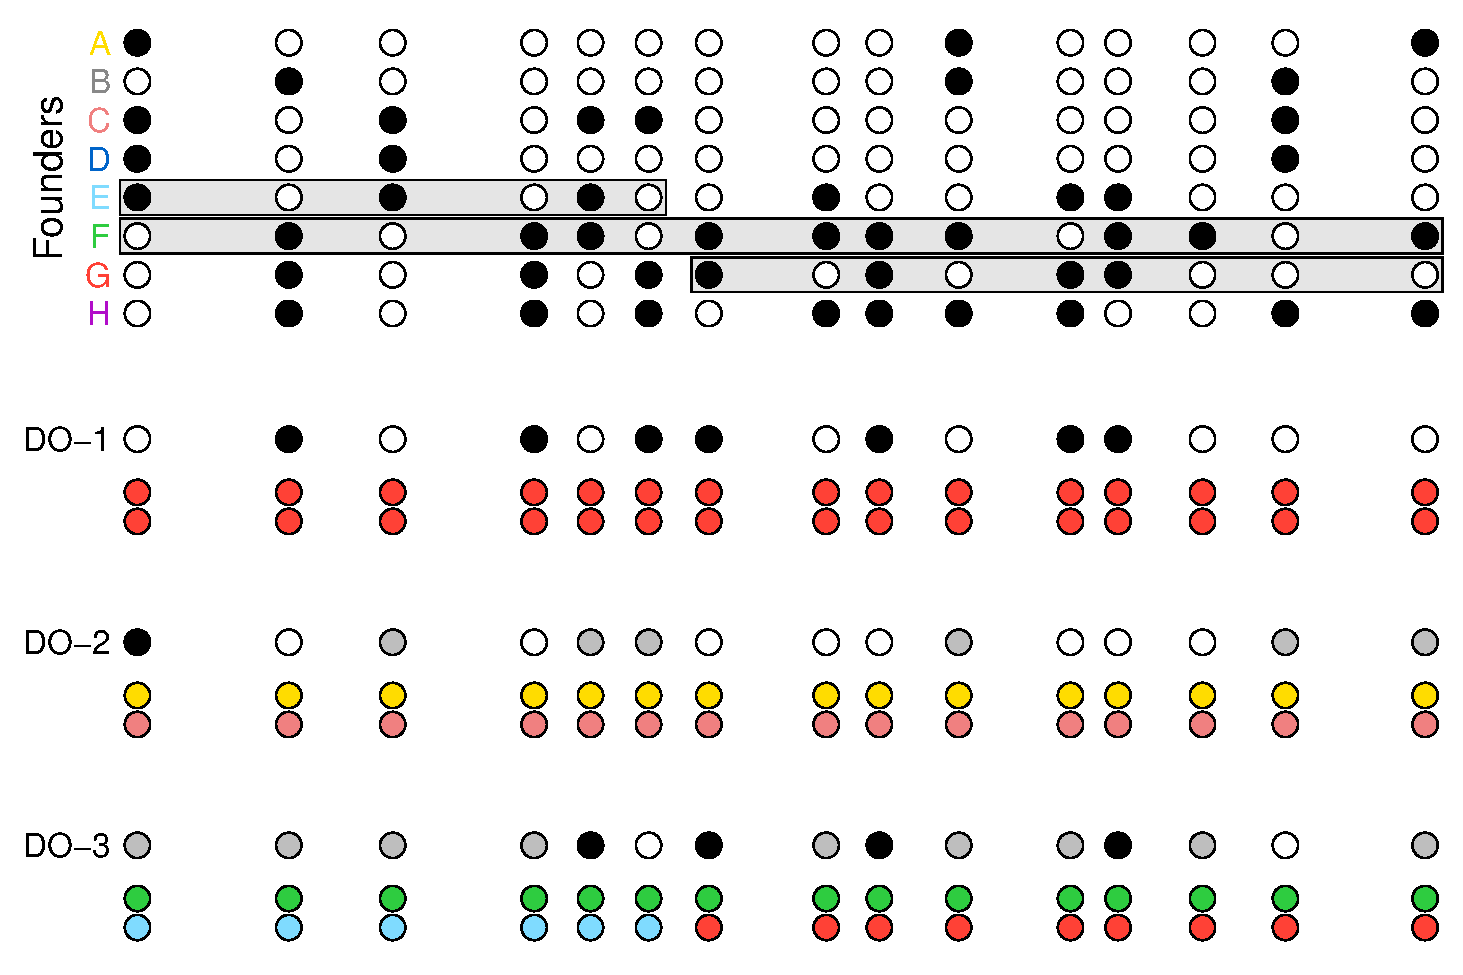
\includegraphics[height=\paperheight,width=\paperwidth]{figures/genoprobsF.pdf}}
		\setbeamertemplate{navigation symbols}{}
    		\begin{frame}[plain]
    		\end{frame}
		
		\usebackgroundtemplate{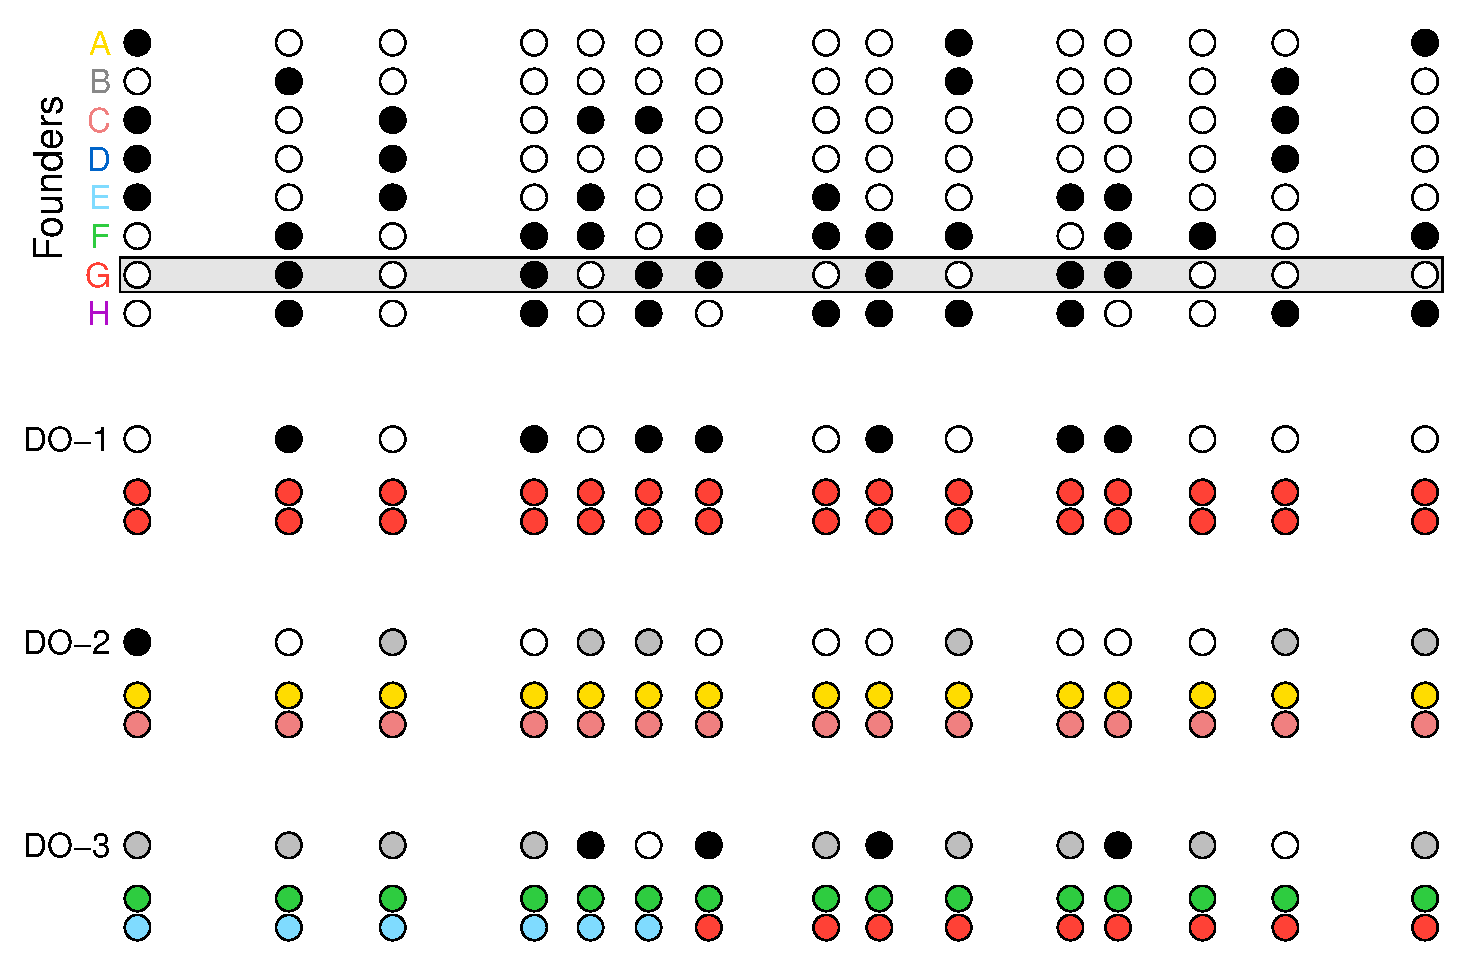
\includegraphics[height=\paperheight,width=\paperwidth]{figures/genoprobs.pdf}}
		\setbeamertemplate{navigation symbols}{}
    		\begin{frame}[plain]
    		\end{frame}
	
		\usebackgroundtemplate{
\includegraphics[height=\paperheight,width=\paperwidth]{figures/white.jpg}}
		\setbeamertemplate{navigation symbols}{}

	\begin{frame}
		\frametitle{Data}
		\vspace{0.3in}
		Two \textit{large} 3D arrays of emission probabilities \\
		
		\vspace{0.25in}

		\begin{itemize}
			\item \texttt{r\textbackslash qtl2} (Broman)
			\item \texttt{DOQTL} (Gatti) \\
		\end{itemize}
		
		\vspace{0.25in}

		\pause $500 \times 120,000 \times 36$ \qquad (Individual $\times$ Markers $\times$ Haplotype)
		
		\vspace{0.25in}
		
		\pause \textbf{How are they different (or the same)}?
	\end{frame}
	
	\begin{frame}
		\frametitle{Inferred Haplotypes}
			INSERT INFERRED HAPLOTYPE IMAGE (BARS)
	\end{frame}
	
	\begin{frame}
		\frametitle{Measure of distance}
		
		\vspace{0.3in}
		\pause For each individual at each marker: \newline
		
		Compute \textit{sum of absolute differences} 
		$$\sum_{i=1}^{36} |p_{1,i} - p_{2,i}|$$
		\pause \textbf{Reduces problems to two-dimensions}: \pause $500 \times 120,000$ \newline
		
		\pause Each entry represents distance between methods
	\end{frame}
		
	
	
\end{document}












